\section{Design Overview}\label{s:design}
\begin{figure}
    \centering
    \begin{subfigure}[b]{0.5\textwidth}
        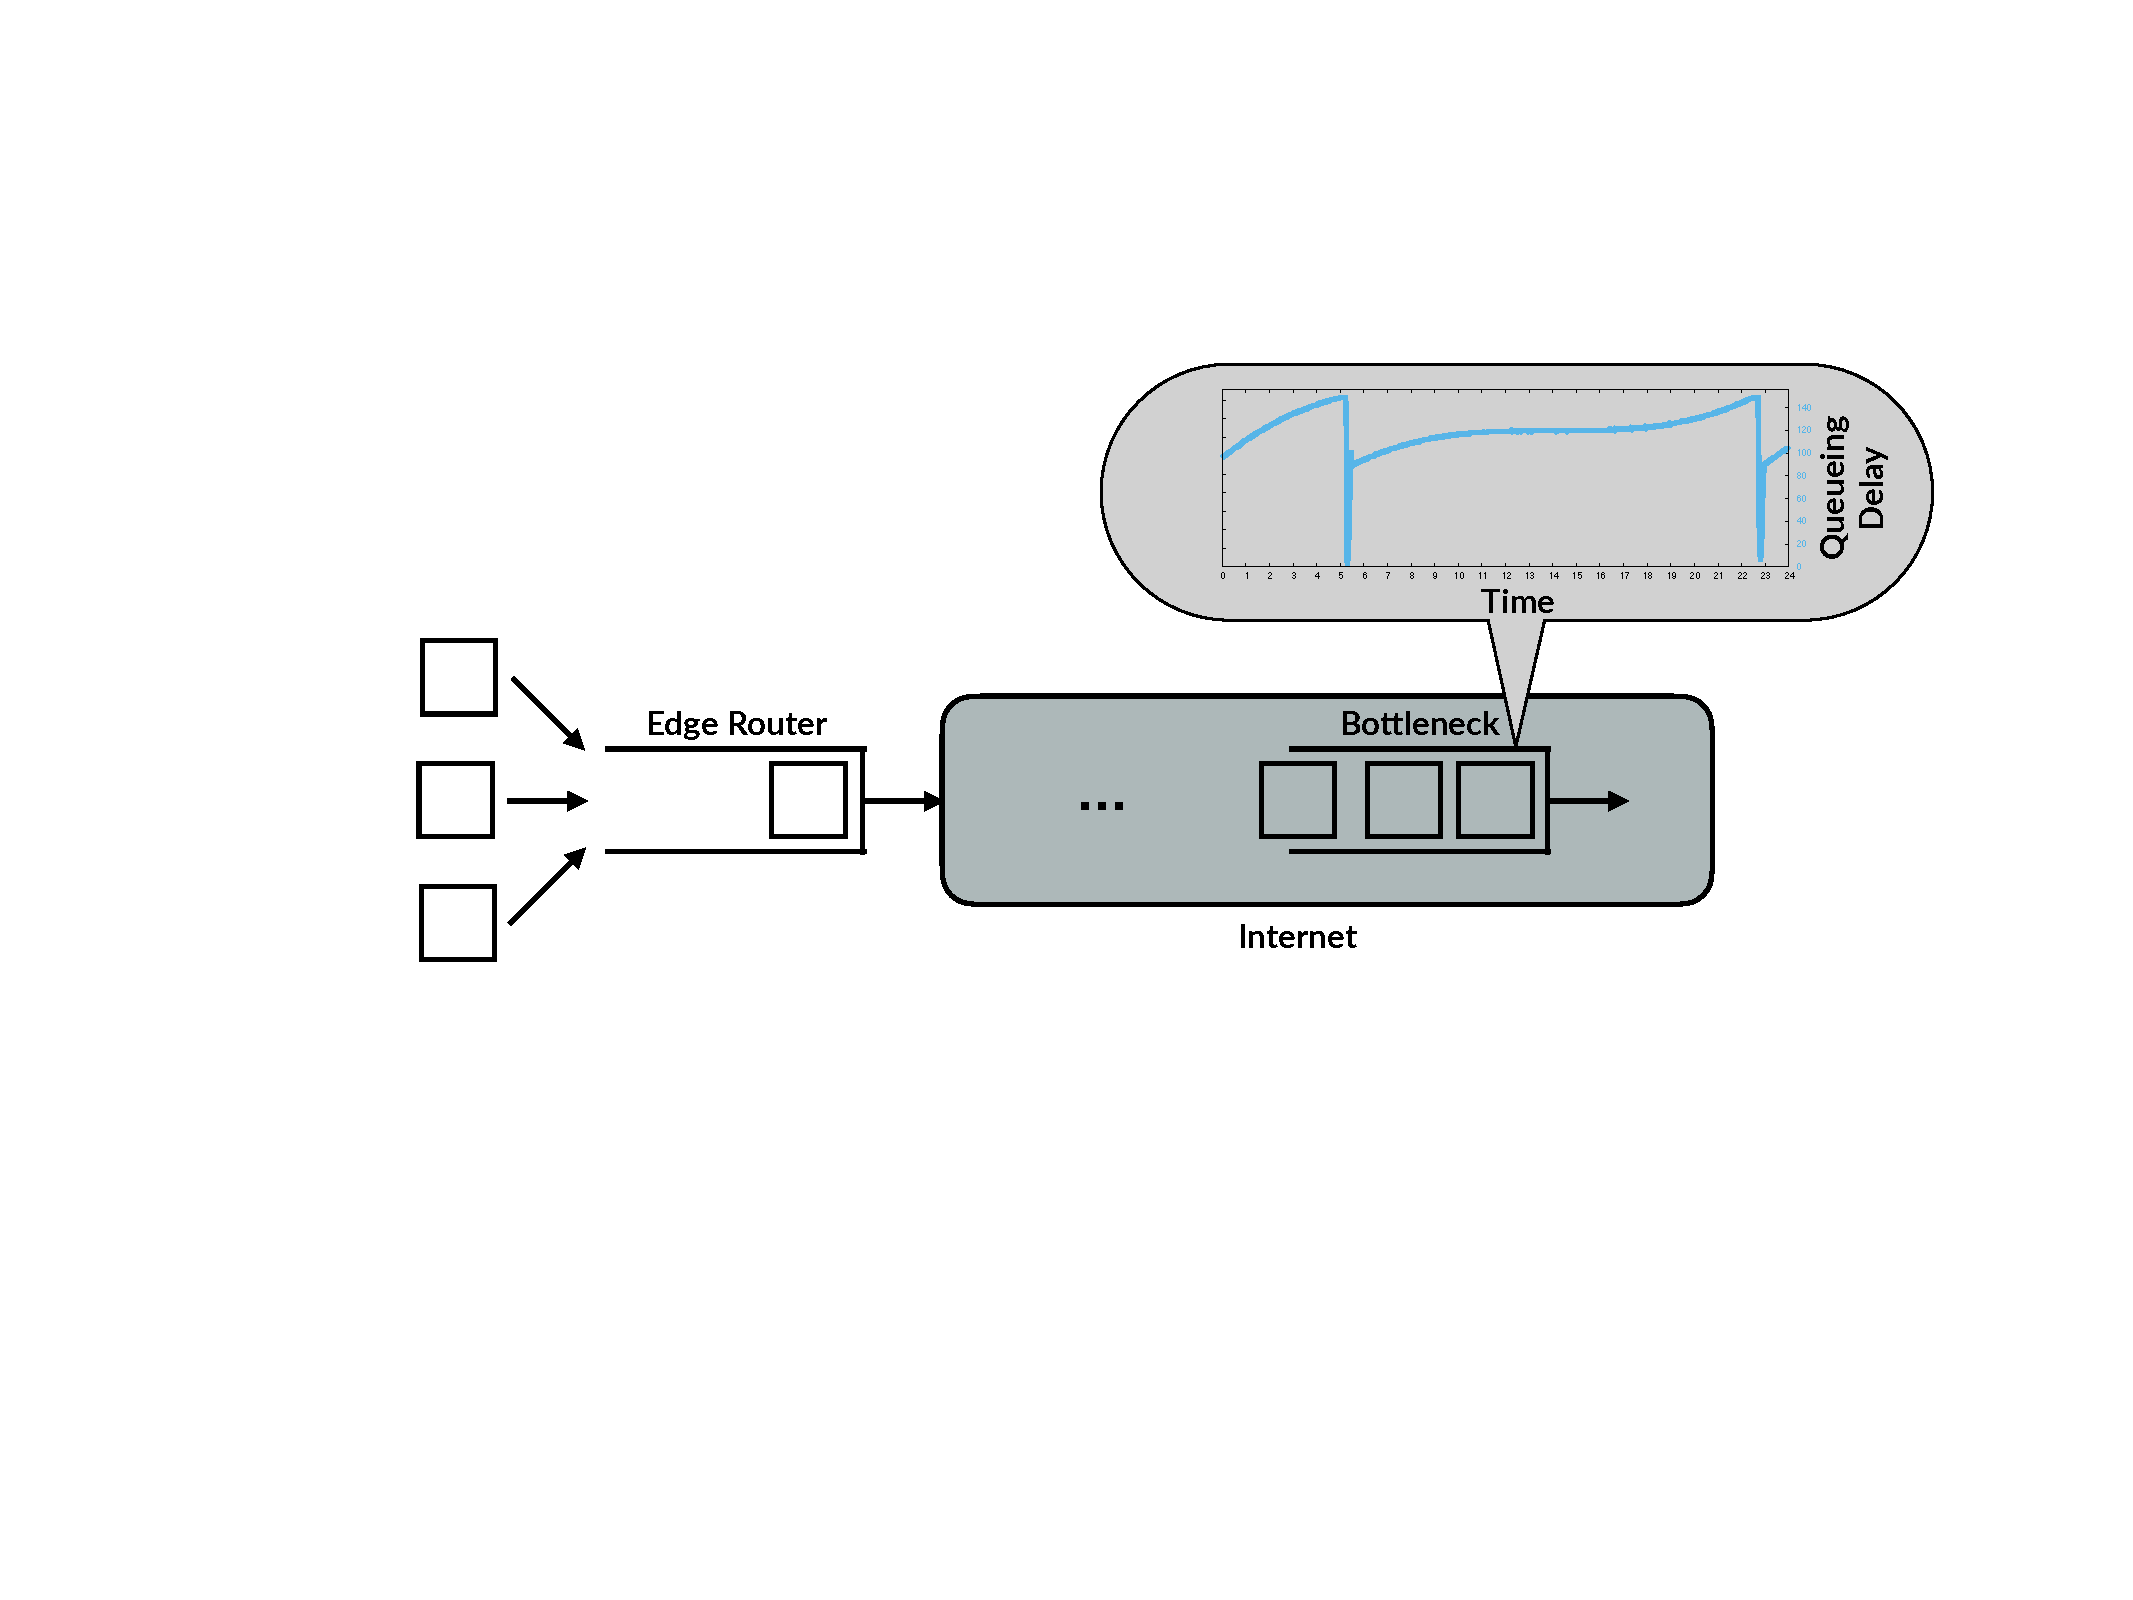
\includegraphics[width=\textwidth]{img/shift-bottleneck-before}
        \caption{Today, large queues can grow on congested routers that are outside the control of a domain.}\label{fig:design:shift-bottleneck:before}
    \end{subfigure}
    \begin{subfigure}[b]{0.5\textwidth}
        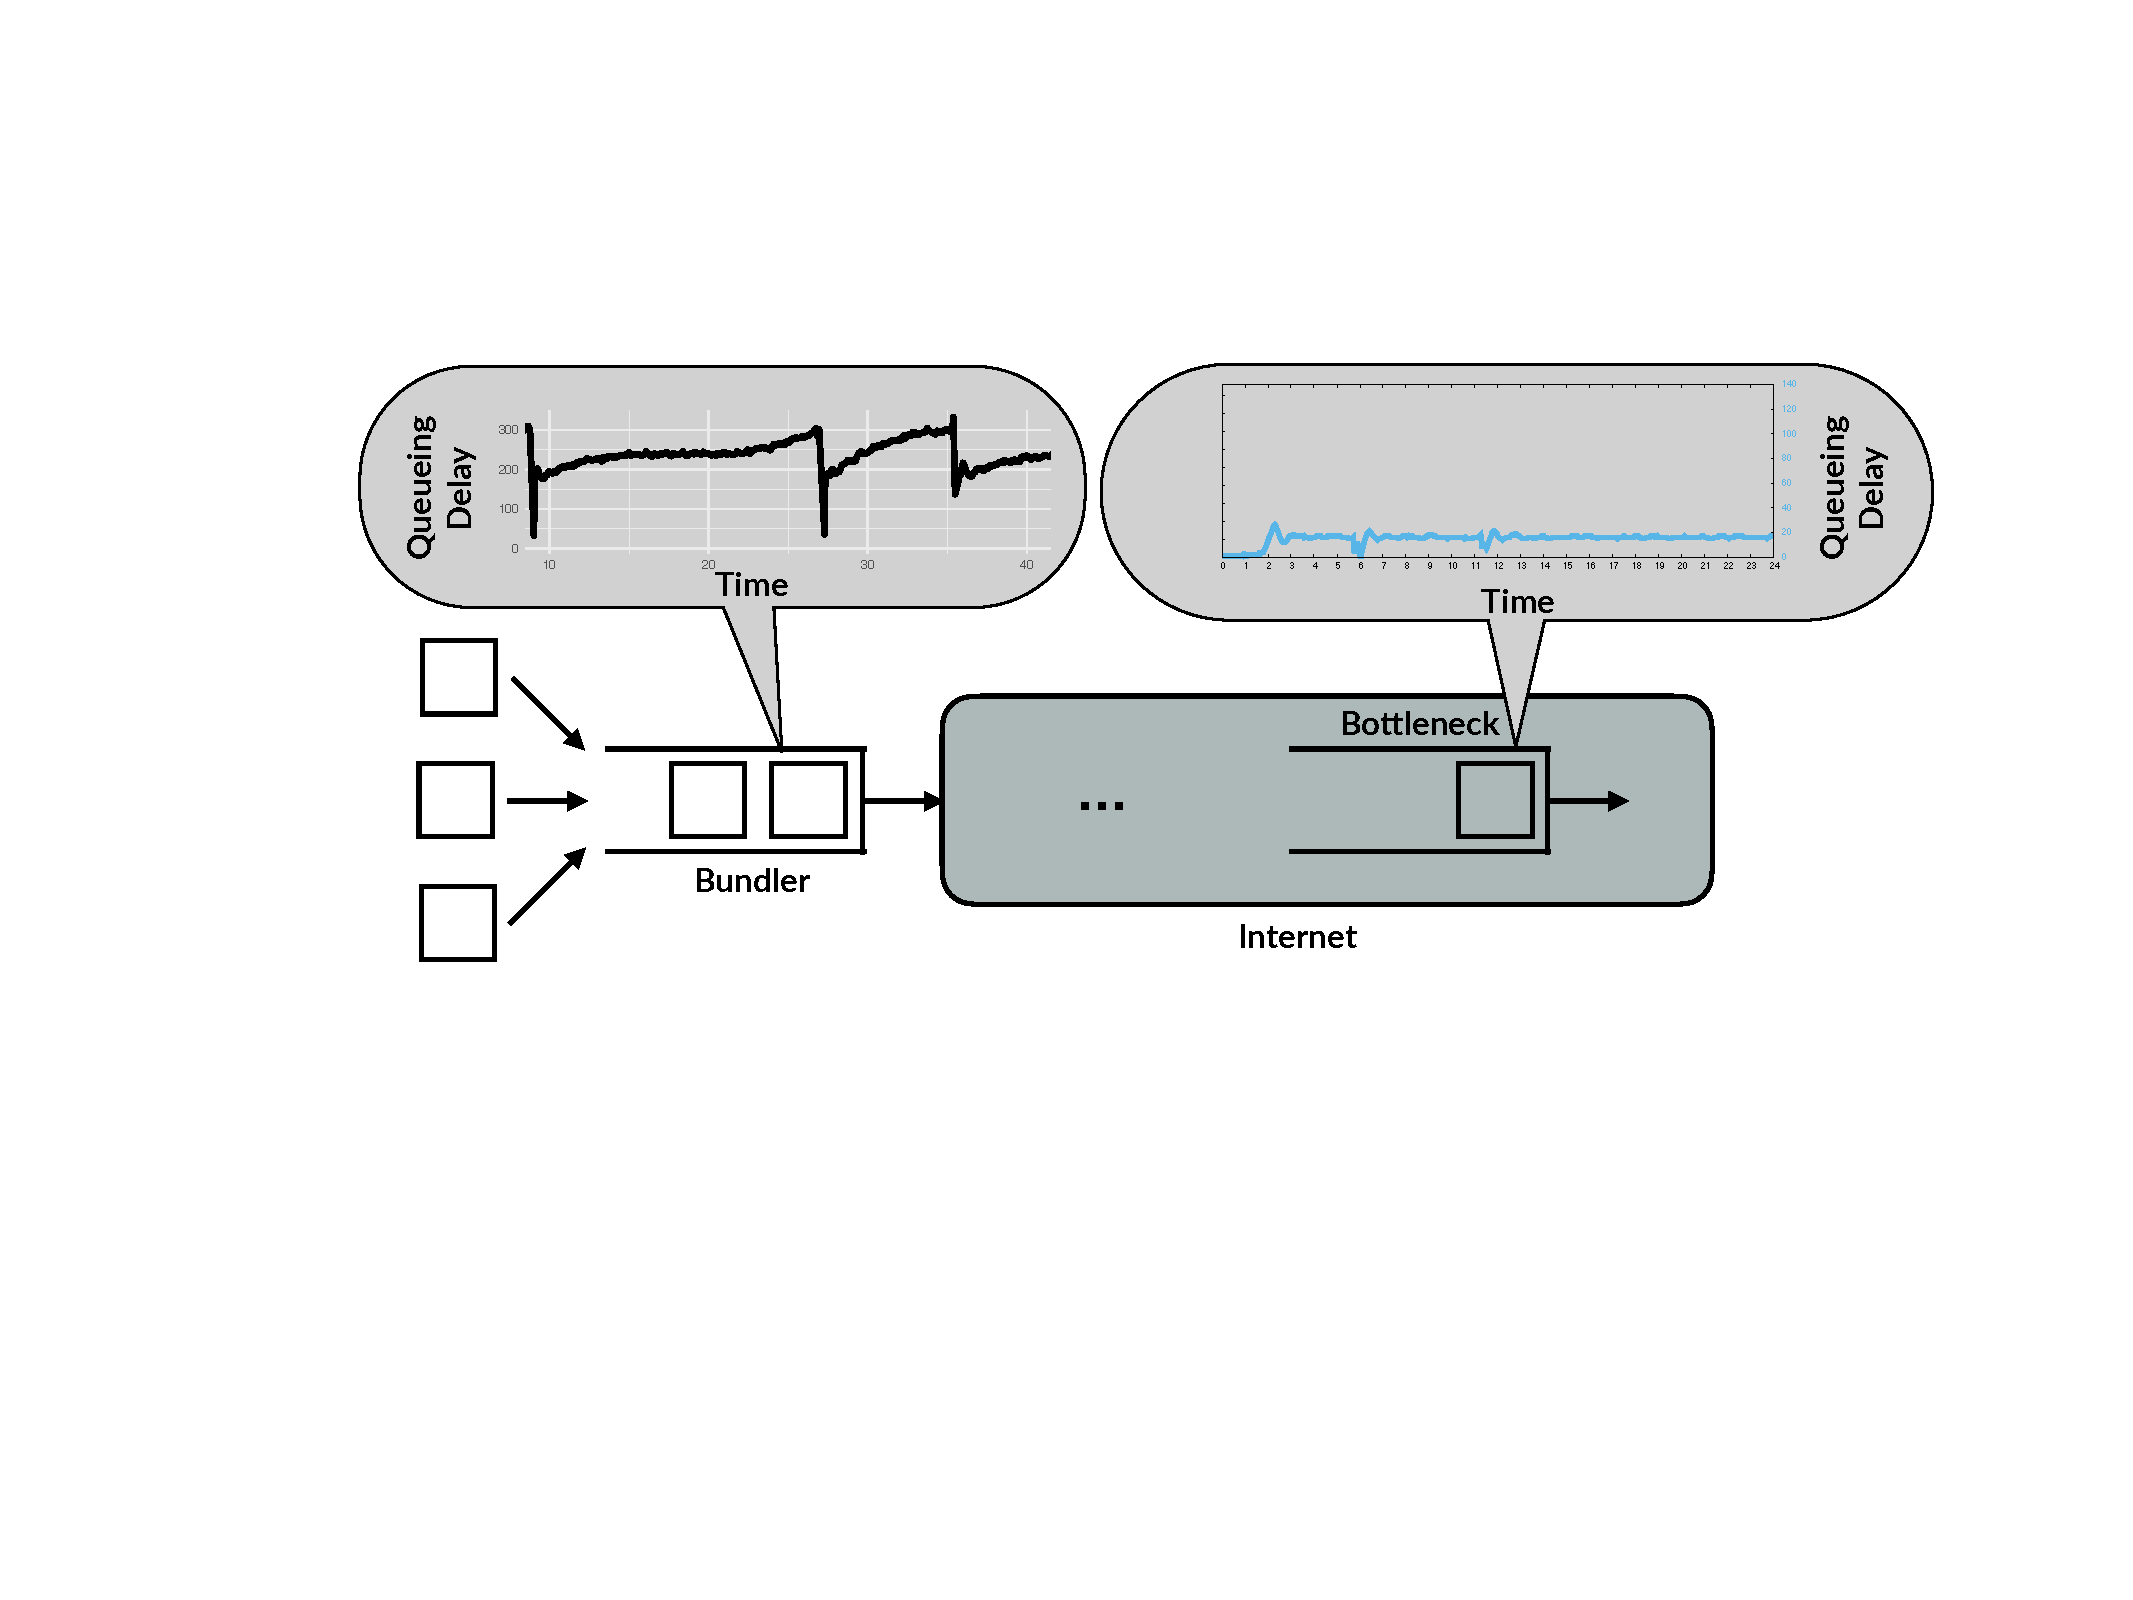
\includegraphics[width=\textwidth]{img/shift-bottleneck-after}
        \caption{\name can \emph{move} the bottleneck using a congestion control algorithm on the traffic aggregate.}\label{fig:design:shift-bottleneck:after}
    \end{subfigure}
    \caption{This illustrative example with a single flow shows how \name can take control of queues in the network. The bubbles show the trend in measured queueing delays at the relevant queue over time. The queue where delays build up can best make scheduling decisions, since that is where there is the most choice between packets to send.}\label{fig:design:shift-bottleneck}
\end{figure}

A \name must have the following properties:
\cut{ % these items could be considered implementation details
    \item It measures congestion control information from the network path.
    \item It enforces a pacing rate determined by a congestion control algorithm. The congestion control algorithm takes as input measurements from the network path, and returns an aggregate rate at which \name should send its component traffic.
}
\begin{enumerate}
    \item It provides a mechanism for scheduling the packets comprising the bundle.
    \item It must be deployable, therefore, it cannot rely on changes in end-hosts.
    \item It must be capable of deployments on the edge of a domain. Therefore, it must also scale to high link rates. As a result, it should not maintain per-connection state -- only per-aggregate state.
\end{enumerate}

\subsection{Shifting the Queues}\label{s:design:shifting}

The key insight of \name is that shifting the queues from the bottleneck to the edge enables scheduling for the aggregate.
Note that \name can only shift (and therefore can only schedule) that component of the bottleneck queue which is self-inflicted; that is, it can only control its own traffic.
\name must therefore decide what fraction of the bottleneck queue it is willing to occupy.
We make a simple, but powerful, observation: end-host congestion control algorithms perform exactly this calculation!
If we run a congestion control algorithm at the \name, it will decide on a fair sending rate for the aggregate as it competes with non-aggregate traffic from other domains.
Component flows will then queue at the \name as their packets are sent at this rate.
Figure~\ref{fig:design:shift-bottleneck} illustrates this method: 
in Figure~\ref{fig:design:shift-bottleneck:before}, packets from the end-hosts queue in a FIFO queue in the network. The FIFO queue at the edge is unoccupied.
In contrast, the \name implementation (described in \S\ref{s:impl}), in Figure~\ref{fig:design:shift-bottleneck:after} maintains low queueing delays at the bottleneck queue by estimating and sending at the bottleneck rate. 
Since component flows, running traditional congestion control algorithms, will probe for bandwidth until they experience loss, they build queues at the \name instead of at the bottleneck.
Since the \name now controls the queues corresponding to the traffic aggregate, it can schedule the packets of component flows.

\cut{
In this section we describe the tradeoffs in the design of a \name.

Bundler is designed to be simple, scalable, and easy-to-deploy.
- Needs to scale to high link rates since it sits on the path and traffic from many hosts will be
passing through it
- Should be simple and possible ot move to hardware for even more scalability
- Must not rely on changes in end-hosts or significant changes to the middlebox in order to 
be practical and readily deployable
- Must be robust to failure scenarios and not cause more harm than good (i.e. if it fails, 
it should at worst make the situation the same as it was before, not any worse)


- To schedule flows, bundler needs to build queues and control the bottleneck
- To control the bottleneck, it needs to perform congestion control
- To perform congestion control, it needs to collect measurements about the state of the network
- It needs at least the sending and receiving rates and RTT 
- It can directly observe the send rate, but the receive rate is known to be difficult to estimate
and an RTT estimate doesn't make much sense

Bundler
Bundler uses two-sided measurements
Bundler does not split connections
Bundler is out-of-band


In order to perform congestion control, \name needs to collect and maintain measurements about 
the current state of the network. State-of-the-art rate-based algorithms such as BBR and Nimbus use
the sending and receiving rates as well as an estimate of the RTT. Although \name can 
directly compute its own sending rate, it can only estimate the receive rate using the timing between received
acknowledgements, which prior work has shown to have limited accuracy~\cite{packet-dynamics, path-properties}.
It would also be difficult to compute a useful estimate of a single RTT representing the entire bundle as each 
flow may experience different sources of latency after traversing the shared bottleneck. We are fundamentally
limited in the accuracy of measurements we can obtain by only observing one side of the bottleneck.
Thus, to obtain more robust and useful measurements, \name actually uses a pair of middleboxes, both
on the network path: one before the bottleneck, and one after, which we refer to as the \textit{\inbox}
and \textit{\outbox}, respectively.

By rate limiting flows in a bundle, we can shift the bottleneck from an intermediate router
to \name itself, and thus allow the queues to build at the inbox. This provides the opportunity
for \name to schedule flows, which is one of \name's key benefits. 

- Since the bottleneck must be between the inbox and outbox, it makes sense to push them as 
close to the sender and receiver as possible to capture as many bottlenecks as possible
- At the same time, the further they are into the network, the more senders and receivers they
can aggregate
- Thus the position should be balanced
- This only works if the bottlebneck is between the inbox and outbox, but if it isn't, it doesn't do any harm

The two middlebox design also allows us to sidestep the problem of determining which flows share
the same bottleneck and thus should be bundled together.  If packets for two different flows are traversing
both the same inbox and outbox on their way from source to destination, 
must 
}

\subsection{Two-sided Measurement}\label{s:design:twosided}
\fc{lock}
In order to perform congestion control, \name needs to collect and maintain measurements about the current state of the network. Traditionally, end-host congestion control has been tightly integrated with end-host packet transmission logic.
\cut{
\begin{outline}
\1 Traditionally, end-host congestion control has been tightly integrated with end-host packet transmission logic.
    \1 Therefore, it traditionally uses a \emph{one-sided} mechanism for measuring congestion control primitives.
    \2 Therefore, it has relied on those measurements that are readily available on end-hosts, \ie the number of in-order packets accounted for by the receipt of an acknowledgement from the receiver.
    \2 Hosts can easily measure the rate at which they send, and the round-trip time.
    \2 However, recent proposals observe~\cite{bbr, sprout, remy, nimbus} that it is often useful to account for the receiver's view of a connection's rate.
        \3 These proposals estimate the received rate at the sender using the timing between received acknowledgements.
        \3 Sender-side only measurements of the bottleneck rate have long been known to have limited accuracy; receiver-side measurements are more accurate~\cite{packet-dynamics, path-properties}.
\1 However, we want a scalable design that does not maintain per-connection state. 
    \2 Tracking acknowledgements requires maintaining this state.
    \2 It also requires path symmetry.
\1 In contrast, we propose a \emph{two-sided} mechanism for measuring network path properties.
    \2 We do this using middleboxes.
    \2 We refer to the middlebox near the sender(s) the \emph{\inbox}, and the middlebox near the receiver(s) the \emph{\outbox}.
    \2 The \inbox is responsible for performing congestion control (and enforcing congestion control decisions) and gathering sender-side measurements.
    \2 The \outbox is responsible for performing measurements on traffic destined for receivers that flows through it.
    \2 One consideration is how to ensure that traffic between the senders and receivers indeed flows through the in-box and out-box, with the prevalence of SDN, something like way-point routing~\cite{waypoint-routing, flowtags} can be used. 
    \2 Also network verification~\cite{veriflow, anteater, reachability} to ensure that traffic indeed traverses in- and out- boxes.
\end{outline}
}

\subsection{What About TCP Proxies?}\label{s:design:prior}
\fc{lock}
\fc{Maybe this belongs in related work instead?}
\cut{
\begin{outline}
\1 An existing approach which could fulfill these design objectives is a TCP Proxy.
    \2 TCP proxies are popular in cellular networks
    \2 They are usually used to shorten the observed round-trip time of a connection, so it can quickly ramp up its sending rate.
    \2 They do this by sending acknowledgements to the sender.  
        \3 This means they must take responsibility for reliable delivery.
    \2 Because TCP proxies take responsibility for reliability, they must implement full TCP stacks.
        \3 As a result, they are difficult to implement in hardware and difficult to scale. \an{maybe mention this later, once it's more clear our design is hardware-compatible?}
    \2 They furthermore remain limited by one-sided measurements.
    \2 They do not allow fate-sharing:
        \3 If a TCP proxy fails, as middleboxes often do~\cite{aplomb}, the underlying connection is broken.
\1 We describe in \S\ref{s:measurement} how a \name can perform precise congestion control measurements without implementing a TCP proxy
    \2 and how to perform these measurements in a fault-tolerant way that preserves fate-sharing.
\end{outline}
}

\subsection{Out-of-band Coordination}\label{s:design:oob}
\fc{lock}
    \cut{
\begin{outline}
\1 A primary consideration for a \name is whether the two gateways should communicate their congestion control measurements \emph{in-band}, by encapsulating packets with \eg a custom UDP header.
\1 Indeed, past approaches to network-assisted congestion control have relied either on encapsulation or custom congestion headers~\cite{xcp, rcp} (probably can cite some cellular thing here).
\1 encapsulation has two drawbacks:
    \2 fault tolerance: if the in-box and out-box fail, as middleboxes often do~\cite{aplomb}, encapsulated traffic flows would also fail. We want to avoid this fate-sharing.
    \2 performance: although modern software switches can achieve high line rates~\cite{netbricks, bess}, they cannot match the performance of hardware. \an{can we say this? could an in-band approach still work with a hardware implementation of the in-box?} 
    \2 load balancing: commonly-deployed ECMP load balancing relies on the 5-tuple of the connection. Encapsulating packets changes the 5-tuple. 
        \3 A naive implementation of encapsulation would simply pick one UDP port, but this would lose all the benefits of load balancing. 
        \3 Instead an implementation would have to carefully set the udp src and dest ports to ensure both that ECMP load balancers in the network still performed correctly, and that the distribution of paths traversed by the encapsulated flows matched those that the unmodified traffic would have traversed without encapsulation.
\1 Therefore, instead, we select an out-of-band approach. In this approach, flows from the senders traverse the network exactly as they otherwise would have. This is nice in terms of the end-to-end principle.
\1 We explain in \S\ref{s:measurement} our measurement methodology
\end{outline}
}

The \inbox and \outbox must communicate in order to share measurements and coordinate actions. 
This communication can either be in-band, which would involve encapsulating packets
at the \inbox with a custom header and then decapsulating them at the \outbox, or out-of-band,
which would not touch any of the actual traffic and send separate packets
An \emph{in-band} approach would involve encapsulating packets at the \inbox with a custom 
header that contains measurement or control information and then decapsulating them at the \outbox.
An \emph{out-of-band} approach 
There are broadly two styles of communication that a \name could use to communicate measurements
and coordinate actions: 

- The inbox and outbox must communicate to coordinate
- Communication can be in band with the traffic we are trying to control or out of band
    - In band involves encapsulating packets with a custom UDP header
    - Out of band does not touch packets and sends separate packets explicitly on a different channel
- Prior work on network assisted congestion control has used encapsulation and/or custom headers 
- This is the most flexible option because you can put whatever you want into the header, but it has a 
a few major drawbacks that violate our design objectives
    1. Adding a header adds overhead, both in terms of the CPU cycles necessary to rewrite each packet
    (as opposed to just passively observing it in the out-of-band case) and in terms of the extra data
    on the wire. This hurts scalability and would be more difficult to implement in hardware.
    2. Bad fault tolerance story -- if either of the boxes fail, which middleboxes often do, 
    all flows currently in bundles would also fail, fate sharing
    3. Messes with ECMP load balancing in the network -- ECMP typically load balances based on five-tuple
    but a naive encapsulation 